\chapter{Troubleshooting}
\label{troubleshooting}

You learn the most through troubleshooting.  However, troubleshooting
can be frustrating when you are tired. You need plenty of gumption and
an open mind. Difficult problems are usually a combination of two or
more problems. So \textbf{do not attempt if you are tired or in a
  hurry}.

Before you start, you need an A3 printed schematic, annotated with
any changes your group may have made.


\section{The scientific method}

Successful troubleshooting requires application of the scientific
method.  First you form a hypothesis about the cause of the problem
and then you test your hypothesis by making observations.  If the
observations do not confirm your hypothesis, you need to revise your
hypothesis and make more observations.

For example, let's say the IMU does not work.  A hypothesis is that
the chip has no power, so you test this by measuring the power supply
voltage at the chip with an \hyperref[oscilloscope]{oscilloscope}.
But why not use a multimeter?  Well, a multimeter only gives the
average value and will not show you that a voltage regulator is
oscillating or if there is a lot of noise.  If the power supply looks
fine, you need another hypothesis, say that the MCU is not outputting
I2C signals.  You then make observations of the I2C signals, with an
oscilloscope, to see if they are changing.  If the waveforms seem
fine, you might hypothesise that the IMU is not configured for the
correct I2C address.  So you then check that the acknowledge bit is
driven low by the IMU.  If there is no acknowledgement, you then check
the address that the IMU is configured for and the address sent over
the I2C bus.  If these match, you might hypothesise that there is a
poor electrical connection.  So you look at the soldering under a
microscope, and so forth.

When forming hypotheses, you need to start with the more likely ones.
Hypothesising that a chip is blown is unlikely unless you observed the
release of magic smoke, noticed that the chip got very hot, noticed an
electrostatic spark, or applied a high voltage, say by putting your
PCB on something conductive.

As you get more desperate, you need more outlandish hypotheses about
what may have gone wrong.  Here, experience helps.  However, the key
is forming a hypothesis based on previous observations\footnote{``Once
  you eliminate the impossible, whatever remains, no matter how
  improbable, must be the truth.'' --- Sherlock Holmes.}.


\section{Reporting software errors}
\label{reporting-software-errors}

A common source of issues is improperly configured software; it is
helpful to catch these errors before getting out the
\hyperref[oscilloscope]{oscilloscope} and probing the hardware. It is
good coding practice to check the return values of library functions
for errors. For mmculib and mat91lib library functions, read the
function's implementation to determine what value they return on
failure. For standard library functions such as \code{printf}, for
example, read the man pages by running \code{man 3 printf} in the
shell or Googling `man printf(3)'. Generally:
%
\begin{itemize}
\item Functions that return a pointer will return a \code{NULL}
  pointer on failure.

\item Functions that return an integer will return 0 on success and a
negative integer on failure.
\end{itemize}

You should add a dedicated error LED to your board that you can flash
in an error state. For example, you could have a panic routine that
flashes the error LED every 400\,ms in an infinite loop:
%
\begin{minted}{C}
static void panic (void)
{
    pio_config_set (LED_ERROR_PIO, PIO_OUTPUT_LOW);
    while(1)
    {
        pio_output_toggle (LED_ERROR_PIO);
        delay_ms (400);
    }
}
\end{minted}
%
Then, say you are initialising a PWM module, you should check to see
if \code{pwm_init} returns a \code{NULL} pointer:
%
\begin{minted}{C}
pwm_t pwm1 = pwm_init (&pwm1_cfg);
if (! pwm1)
    panic ();
\end{minted}
%
You can also use the USB serial interface to report errors. However,
try to keep your panic routine simple to minimise the risk of an error
occurring during its execution!

It is even better if you can spot software bugs before programming
your board. Make sure you compile with the \code{-Wall} flag and
resolve any compiler warnings before programming.

\section{Oscilloscope}
\label{oscilloscope}

The best tool for debugging an embedded system is an oscilloscope.

\begin{enumerate}
\item Use $\times$10 probes\footnote{These attenuate the signal by a
  factor of 10 but reduce the probe capacitance by a factor of 10.} to
  reduce loading on the circuit.

\item Use the correct probes for the scope so that they can be
  automatically detected.

\item Compensate the probes by clipping to the probe test signal on
  the scope and adjusting the variable capacitor in the probe to
  ensure a square wave without undershoot or overshoot. This is one of
  the few times you are allowed to use the autoscale button!

\item Check that the probe gains are correct; they should by $\times
  10$ for $\times 10$ probes.

\item Hypothesise what you should expect to observe and set up the
  oscilloscope accordingly.  Pushing the auto-set button only works
  for AC or DC signals and is hopeless for transient signals, such as
  I2C bus waveforms.  For transient signals, use normal mode triggering.

\end{enumerate}

\begin{figure}[!h]
  \centering
  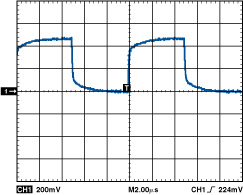
\includegraphics[width=0.3\columnwidth]{figs/probe-undercompensated}
  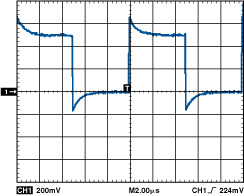
\includegraphics[width=0.3\columnwidth]{figs/probe-overcompensated}
  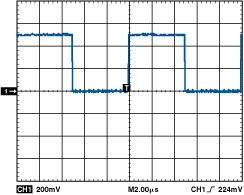
\includegraphics[width=0.3\columnwidth]{figs/probe-compensated}
  \caption{Oscilloscope probe compensation: under, over, and proper.
    From
    \url{http://www.analog.com/library/analogdialogue/archives/41-03/time_domain.html}.}
\end{figure}


\subsection{Normal mode}
\label{normal-mode}

This mode is for measuring transient or non-repetitive signals, such a
serial bus waveforms. It will only refresh the display if a trigger
event is detected.  You need to adjust the trigger level.

It is useful to increase the trigger holdoff to prevent triggering on
multiple edges of a waveform.  By default, it is set to a ridiculously
small value.

\subsection{Auto mode}
\label{auto-mode}

This mode is for measuring AC or DC signals. It is like normal mode
but if it does not detect a trigger it will automatically refresh the
display.


\subsection{Interpreting digital signals}

In theory a digital signal will be either high or low.  In practice,
it is an analogue signal and you will see the rise/fall transitions,
over/undershoot, interference due to crosstalk, and other noise.  The
oscilloscope has a limited bandwidth and thus the displayed signals
are low-pass filtered.

\begin{description}
  \item[The signal does not go fully high] This is likely to be due to
    a resistive load connected to ground.

  \item[The signal does not go fully low] This is likely to be due to
    a resistive load connected to VDD.

  \item[The signal slowly changes] The signal output is likely to be
    tri-stated.

  \item[The waveform sometimes goes fully high or fully low but
    sometimes has intermediate values] This is likely to be due to two
    outputs driving the same signal that are fighting each other.
\end{description}



\section{SAM4S not detected by OpenOCD}
\label{sam4s-not-detected-by-openocd}

OpenOCD communicates with the SAM4S using either JTAG or SWD serial
interfaces.  The following assumes SWD as used by the ST-link
programmer.  SWD is a two wire bus with a clock signal and a
bi-directional data signal.


\subsection{SAM4S never detected by OpenOCD}

If the SAM4S has been previously programmed, say it has been removed
from a previous project, \hyperref[erasing-flash-memory]{erase flash
  memory} and try reconnecting with OpenOCD.

%
\begin{enumerate}
\item
  Check orientation of the SAM4S (the small circle marks pin 1).

\item
  Check 3.3\,V and 1.2\,V power rails; none of them are optional.  The
  ST-link programmer should provide 3.3\,V and the internal regulator
  in the SAM4S provides 1.2\,V.

\item
  Check the serial wire debug (SWD) signals, see
  \protect\hyperref[debugging]{debugging serial wire debug (SWD)}.
  Note, there are two variations of the ST-link programmer.

\item
  Check soldering of the SAM4S pins under a microscope.  Giving
  each pin a push with a sharp spike can reveal a poorly soldered joint.

\end{enumerate}


\subsection{SAM4S stops being detected by OpenOCD}

If OpenOCD stops working after a program is loaded,
\protect\hyperref[checking-the-crystal-oscillator]{check the crystal
  oscillator}.  This is because the crystal oscillator is selected for
the SAM4S clock when a program starts to run.  Before the SAM4S is
programmed, it uses an internal RC oscillator.

If this does not work, \hyperref[erasing-flash-memory]{erase flash
  memory} and reprogram the SAM4S with a LED flash program.  If this
works, you may have something wrong with your program.


\subsection{Erasing flash memory}
\label{erasing-flash-memory}

\begin{enumerate}
\item Connect the ERASE pin to 3.3\,V.

\item Re-start OpenOCD.

\item Re-enable \hyperref[booting-from-flash-memory]{booting from
  flash memory}.
\end{enumerate}


\subsection{Debugging serial wire debug (SWD)}
\label{debugging-serial-wire-debug-swd}

You will need a scope for this.  Hopefully you will have test-points
for the \sig{SWCK} and \sig{SWD} signals.

\begin{enumerate}
\item Check the \sig{SWCK} signal.  \program{OpenOCD} periodically
  polls to see if the SAM4S is alive.  These occur every 100\,ms, see
  \reffig{openocd-poll}.  OpenOCD polls less often when it does not
  get a response. The period increases to 6.3\,s.

\item Zoom in on the \sig{SWCK} signal.  Each spike should look like a
  clock signal.  If it is not periodic, you may have the \sig{SWD} and
  \sig{SWCK} signals transposed\footnote{There are two versions of the
    ST-link programmer.  They look identical!}.

\item Check the \sig{SWD} signal.  If the SAM4S responds, the waveform
  seen in \reffig{openocd-response} should be observed on the
  \sig{SWD} pin.  Note, you will need to zoom in on the waveform.
\end{enumerate}


\begin{figure}[!h]
\centering
\includegraphics[height=2.60417in]{figs/OpenOCDTimingGood.png}
\caption{OpenOCD polls every 100\,ms while connected.  Note, zooming
  in on the spikes reveals serial data packets.}
\label{fig:openocd-poll}
\end{figure}

\begin{figure}[!h]
\centering
\includegraphics[height=2.60417in]{figs/OpenOCDPollingGood.png}
\caption{\sig{SWD} signal when there is a response from the SAM4S.
  The decaying waveform at the end occurs when the pin is tri-stated.}
\label{fig:openocd-response}
\end{figure}


The common problems are:
%
\begin{itemize}
\item No power for SAM4S, 3.3\,V and 1.2\,V.  The 3.3\,V should be
  supplied by the ST-link programmer and the SAM4S internal regulator
  produces 1.2\,V.

\item The \sig{SWD} and \sig{SCK} signals are transposed.  Note, there
  are two variants of the ST-link programmer with different pin-outs!

\item The \sig{SWD} and \sig{SCK} pins are not correctly soldered.
  Check these signals with a scope on the pins of the SAM4S.

\item The SAM4S has been programmed to use the crystal oscillator but
  it is not running, see
  \protect\hyperref[checking-the-crystal-oscillator]{checking the
    crystal oscillator}.
\end{itemize}



\subsection{Checking the crystal oscillator}
\label{checking-the-crystal-oscillator}

When the SAM4S is first powered up it uses an internal RC oscillator.
However, when a program is loaded, the code before main is called
switches the SAM4S to use the main oscillator that uses the external
crystal.  If there is a problem with the crystal oscillator the SAM4S
will not run since it has no clock.  Moreover, \program{OpenOCD} will
then fail to communicate with the SAM4S.

\begin{figure}[!h]
\centering
\includegraphics[height=2.60417in]{figs/ClockSignal.png}
\caption{12\,MHz clock sine wave measured on the XOUT pin.}
\label{fig:xout}
\end{figure}

\begin{figure}[!h]
  \centering
  \mtodo{Add scope picture of CPU clock signals when not working}
  \caption{Oscillator waveform when not working.}
\end{figure}

\begin{enumerate}
\item Connect a scope pin to the \sig{XOUT} pin. A 12\,MHz sinewave
  should be visible, see \reffig{xout}.

\item If there is no sinewave:

  \begin{enumerate}
  \item Measure the voltage on the \sig{VDDPLL} pin of the MCU with a
    scope. This should be 1.2\,V to power the oscillator.

  \item Check the bypass capacitors across the crystal.  These should
    be approx. 20 pF.

  \item Check the \sig{XIN} and \sig{XOUT} solder connections under a
    microscope.
  \end{enumerate}
\end{enumerate}


\subsection{Checking the CPU clock}
\label{checking-the-clock}

The SAM4s has multiple clock sources:

\begin{enumerate}
\item
  Internal fast RC oscillator (this is selected when the SAM4S is first
  ever used).
\item
  Internal slow RC oscillator (this can be selected to save power).
\item
  Main oscillator using external crystal (this is selected when you
  run a program).
\end{enumerate}

The SAM4S uses a phase-locked-loop (PLL) to multiply the frequency of
the clock source to provide the CPU clock.  When a program is loaded,
the SAM4S is configured so that the 12\,MHz crystal oscillator
frequency is multiplied by 16 to 192\,MHz by the PLL and then divided
by 2 to provide the 96\,MHz CPU clock\footnote{The CPU can run at
  speeds up to 120\,MHz by choosing \code{MCU_PLL_MUL} and
  \code{MCU_PLL_DIV} in \file{target.h}.  The USB peripheral needs to
  run at 48\,MHz so either the CPU clock needs to be a multiple of
  48\,MHz or the second PLL needs to be configured for the USB
  peripheral.}.

\begin{enumerate}
\item Sometimes the PLL will run without a clock source and thus will
  generate an unexpected frequency.  The clock frequency can be
  checked by connecting a scope to a peripheral pin that generates a
  clock, e.g., PWM, SCK, TXD, and programming the peripheral.  For
  example, use the \hyperref[pwm-test]{PWM test} program.

  Alternatively, the PLL frequency can be checked using the OpenOCD
  \code{at91sam4 info} command, see
  \hyperref[system-information]{system information}.  Note, the
  reported frequencies are not accurate.

\item The PLL requires a well regulated power supply.  Check that the
  100\,nF capacitor is not too far from the \sig{VDDPLL} pin.
\end{enumerate}


\section{LED testing}
\label{debugging-LED}

The most common reason why an LED does not work is that you have
incorrectly specified its PIO pin in the \file{target.h} file (see
\protect\hyperref[configuration]{configuration}).

An active-high LED should faintly glow before the SAM4S is first
programmed.  This is due to the internal pullup resistors on each PIO
pin.  If the LED does not glow, check its orientation.

If the LED still does not work, use an oscilloscope to check that the
PIO pin is correctly driven.


\section{USB serial}
\label{debugging-usb}

USB is a complicated protocol and there are many possibilities why it
does not work.  First check your hardware by
\hyperref[erasing-flash-memory]{erasing flash memory} and connecting
the USB to a PC.  If a new USB device is detected, your hardware is
correct\footnote{You may have a poorly soldered connection that gives
  intermittent operation.}.  Note, you will then need to re-enable
\hyperref[booting-from-flash-memory]{booting from flash} before
re-loading your program.

If the hardware does not work:
%
\begin{enumerate}
  \item Check that the USB cable is not power-only, say by using a
    known good cable.

  \item
    Check that the USB termination resistors are 27\,ohms.

  \item Check the USB connector pins and the SAM4S USB pins under a
    microscope.  If they move if you push them with a sharp-pointy
    thing, resolder.

  \item
    Check that the USB signals are not transposed.

  \item Check the crystal oscillator is running at 12\,MHz, see
    \protect\hyperref[checking-the-crystal-oscillator]{checking the
      crystal oscillator}.

  \item Check that the CPU is running at 96\,MHz, see
    \protect\hyperref[checking-the-clock]{checking the CPU clock}.

  \item Try an unmodified test program in case you have introduced a
    coding error.
\end{enumerate}

If the USB serial connection drops characters:
  %
 \begin{itemize}
 \item Add a delay before sending data, e.g., \code{delay_ms (100);}.
   This is because the driver takes a while to set up the connection
   after the USB cable is plugged in.  If you try to send some data
   during this time, the data gets stored into a ring buffer for later
   transmission.  However, the ring buffer is not large and once it is
   filled, the USB serial driver will drop characters.
 \end{itemize}


\section{Motors}
\label{motors-testing}

For the motors to work:
%
\begin{enumerate}
\item The H-bridge must be correctly configured.
\item The PWM signals must be correctly generated.
\end{enumerate}


\subsection{Testing the H-bridge}
\label{testing-the-h-bridge}

\begin{enumerate}
\item The \sig{nFAULT} pin should be high.  Note, this is an
  open-drain pin and requires a pullup resistor to 3V3 to make it
  work.  Without this resistor, this pin will always read low, fault
  or no fault.  If this is connected to the SAM4S, it will be pulled
  up by default.

\item The \sig{nSLEEP} pin needs to be high to enable the chip.

\item Check that the capacitor connected to the \sig{INT} pin is
  2.2\,$\mu$F and not 2.2\,nF.

\item Check the \sig{AIN1}, \sig{AIN2}, \sig{BIN1}, \sig{BIN2} pins.
  If you see DC 2\,V, this is due to the signal not being configured
  as an output on the SAM4S; the internal pullup of the SAM4S forms a
  voltage divider with the internal pulldown of the H-bridge chip.

\item Check that \sig{AINSENSE} and \sig{BINSENSE} are connected
  directly to ground or to ground via a small resistor if you want
  current limiting.
\end{enumerate}


\subsection{Debugging PWM}
\label{debugging-pwm}

If PWM does not work:

\begin{enumerate}
\item
  Check the SAM4S pin since not every pin can be a PWM signal.  The
  SAM4S can generate four independent hardware PWM
  signals\footnote{And the complementary output.}. See
  \wfile{mat91lib/pwm/pwm.c} for a list of supported PIO pins.  Note,
  \pin{PA16}, \pin{PA30}, and \pin{PB13} are different options for
  PWM2.

\item
  Check the definition in the configuration file \file{target.h}.
\end{enumerate}

If the PWM frequency is wrong:

\begin{enumerate}
\item
  Check the clock frequency, see
  \hyperref[checking-the-clock]{checking the clock}.
\item
  Check your program.
\end{enumerate}

If the PWM duty is wrong:

\begin{enumerate}
\item
  Check your program. There are two ways to set the duty cycle with
  mat91lib's PWM module: (1) setting the \code{duty} field of the
  \code{pwm_cfg_t} struct using the \code{PWM_DUTY_DIVISOR} macro and
  passing the duty cycle as a percentage or (2) setting the
  \code{duty_ppt} field of the \code{pwm_cfg_t} struct as an integer
  in parts per thousand (e.g., 1000 = 100\% duty cycle; 50 = 5\% duty
  cycle). Setting the latter field will override the former. See the
  definition of \code{pwm_cfg_t} in \wfile{mat91lib/pwm/pwm.h}.
\end{enumerate}

\begin{figure}[!h]
\centering
\includegraphics[height=2.60417in]{figs/PWM_2.png}
\caption{Two PWM signals at 1\,kHz and 10\,kHz.}
\end{figure}


\section{IMU}
\label{imu}

For the IMU to work:
%
\begin{enumerate}
\item The IMU chip must be correctly configured.
\item The I2C bus must be working.
\end{enumerate}


\subsection{IMU checking}
\label{checking-IMU}

\begin{enumerate}
\item Check the I2C bus (see \hyperref[debugging-i2c]{debugging I2C}).
\item Check the auxiliary I2C bus signals are not connected on the IMU
  (otherwise the magnetometer will not respond).
\item Check \sig{nCS} on the IMU is pulled high.
\item Check \sig{FSYNC} on the IMU is pulled low.
\item Try pressing on a side of the IMU with a fingernail to see if it
  starts working; you might have a dry joint.  Otherwise look under
  the microscope at the pins of the IMU and touch them up with a
  soldering iron if necessary.
\item Check that you are using the correct I2C address corresponding
the the state of the AD0 pin (see datasheet).
\end{enumerate}


\subsection{Debugging I2C}
\label{debugging-i2c}

\begin{enumerate}
\item
  I2C/TWI requires external pull-up resistors for the clock (TCK) and
  data (TDA) signals.  Use a scope to look at the signals
  \pin{TWCK/SCL} and \pin{TWD/SDA}.  If the rise times are too slow so
  that the high voltage level is not 3.3\,V, the resistors are too
  large.
\item
  TWI channel 1 (TWI1) uses \pin{PB4} and \pin{PB5}. However, these
  are configured on boot as JTAG pins. You can disable this, see
  \hyperref[disabling-jtag-pins]{disabling JTAG pins}.
\end{enumerate}

The oscilloscopes in the ESL can be configured to trigger on I2C%
\footnote{They also support other serial protocols including SPI and
UART.} frames and automatically decode and display the contents of
each frame. Press the `Protocol' button on the scope then use the
touch screen to change the protocol to I2C. You will require a probe
each for the data and clock signals: touch the `Trigger' button in the
protocol menu to configure which channel corresponds to which signal.
See \reffig{i2c-ack} and \reffig{i2c-noack} for examples.

\begin{figure}[!h]
  \centering
  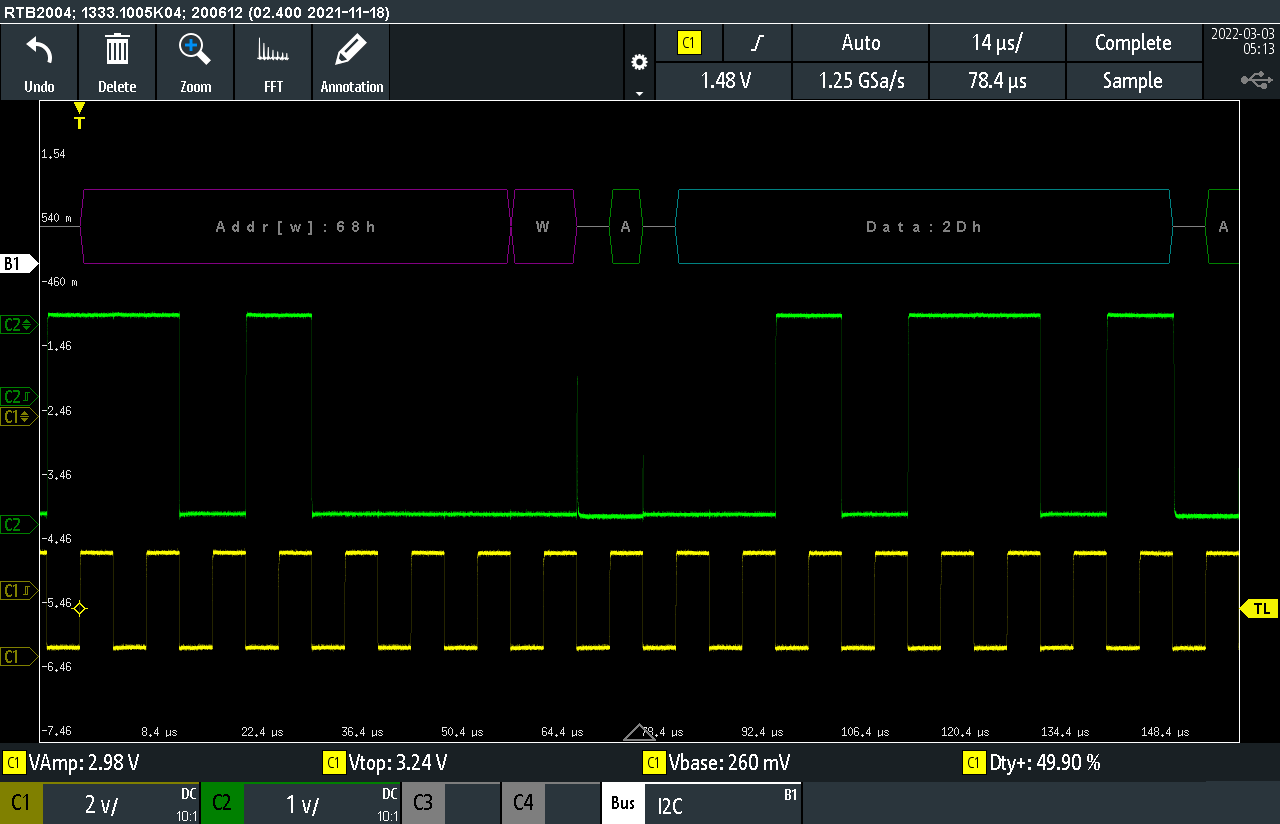
\includegraphics[width=\linewidth]{figs/i2c-ack.png}
  \caption{I2C signals with acknowledgement; the green trace is
  \code{TWD/SDA} and the yellow trace is \code{TWCK/SCL}.}
  \label{fig:i2c-ack}
\end{figure}


\begin{figure}[!h]
  \centering
  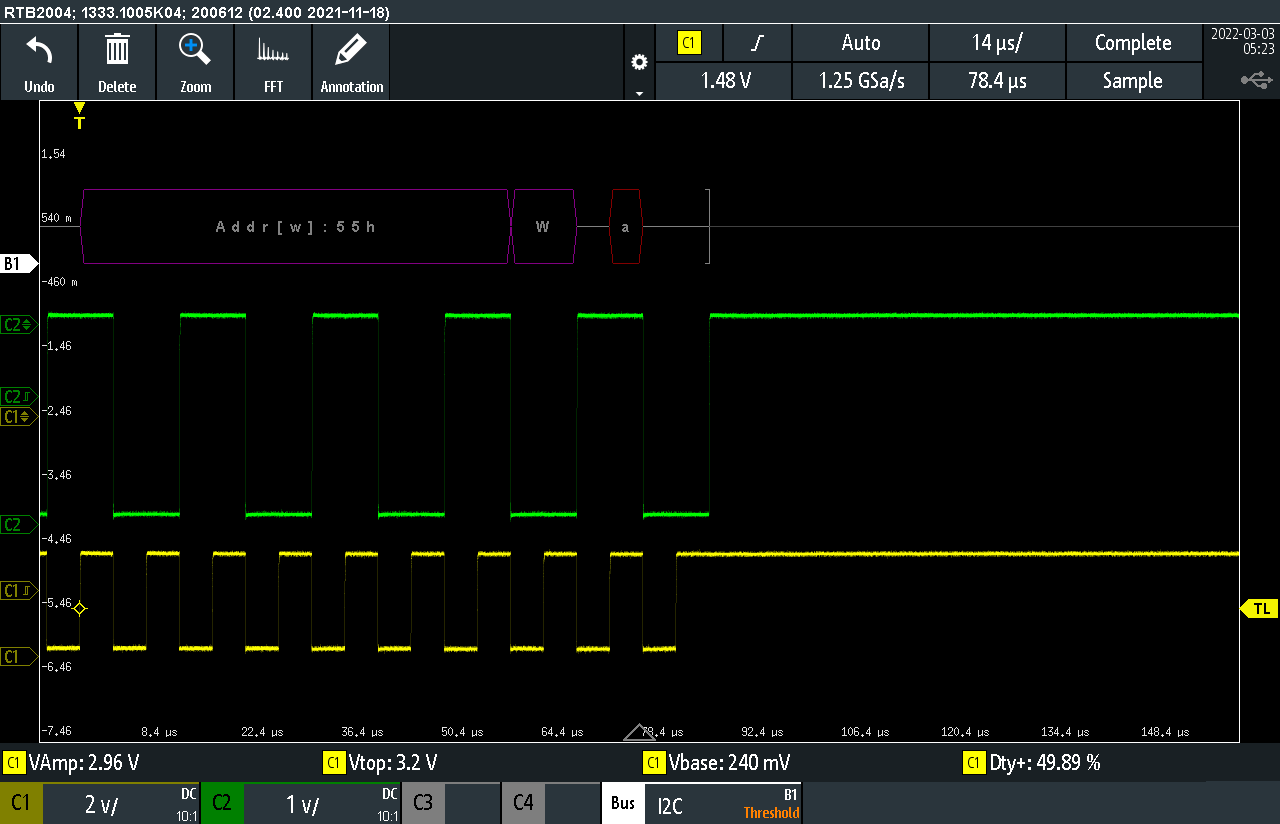
\includegraphics[width=\linewidth]{figs/i2c-noack.png}
  \caption{I2C signals with no acknowledgement; the green trace is
  \code{TWD/SDA} and the yellow trace is \code{TWCK/SCL}.}
  \label{fig:i2c-noack}
\end{figure}


\section{NRF24L01+ radio}
\label{nrf24l01-radio}

For the radio to work you need:

\begin{enumerate}
\item No ground planes near the antenna\footnote{You might have to
  mount the radio vertically.}.

\item A working SPI interface.

\item The correct channel and address.

\item A well filtered power supply for the radio, see \reffig{radio-filtering}.

\item A channel with little interference (note, some channels are
  shared with WiFi and Bluetooth and may be less reliable).
\end{enumerate}

If nothing works, check:

\begin{enumerate}
\item
  For transmission the CE pin should be low; for reception the CE pin
  should be high.
\item
  Check that the SPI clock SCK, MOSI, and MISO signals are driven when
  the radio is configured (note, the MISO signal is tristate when CS is
  high).
\item
  Check that the SPI CS signal is driven low for each transmitted byte.
\end{enumerate}

If the radio transmits but not receives, check:

\begin{enumerate}
\item
  The IRQ pin is driven low (this indicates that a packet has been
  received).
\item
  The power supply. The radio requires a well filtered power supply
  otherwise the range will be limited on reception. Preferably, the
  device should have its own 3V3 regulator with a low-pass RC filter
  comprised of a series resistor and large capacitor (say 22\,$\mu$F)
  or a low-pass LC filter made with a ferrite bead and capacitor.
\end{enumerate}

\textbf{Note}, by default the radio waits for an auto-acknowledgement
from the receiver device. This acknowledgement is performed in hardware.
If no acknowledgement is received, it retries for up to 15 times. The
auto-acknowledgement and number of retries can be configured in
software.

\subsection{Checking the radio power supply}
\label{checking-the-radio-power-supply}

\begin{figure}[!h]
  \centering
  \mtodo{Add scope picture of expected radio power supply voltage}
  \caption{Waveform showing radio power supply voltage.}
\end{figure}


\subsection{Debugging SPI}
\label{debugging-spi}

Check:
%
\begin{enumerate}
\item The device chip select signal is driven low.
\item The \pin{SCK} signal toggles while the chip select is low.
\item The \pin{MOSI} signal does something while the chip select is low.
\end{enumerate}
%
The \pin{MISO} signal is usually tri-state and is driven by the
device when the chip select is low.

The SPI standard is rather loose and there are four modes to confuse
the unwary; these are due to two clock polarity modes and two clock
phase modes.  When using the wrong mode, the read data can be out by a
bit or unreliable.

\begin{figure}[!h]
  \centering
  \mtodo{Add scope picture of SPI signals}
  \caption{SPI signals.}
\end{figure}


\subsection{Debugging ADC}
\label{debugging-adc}

If the ADC does not work:
%
\begin{enumerate}
\item
  Check the SAM4S pin since not every pin can be an ADC input.

\item
  Check the definition in the configuration file \file{target.h}.

\item
  Check that the SAM4S \sig{VDDVREF} pin is 3.3\,V.

\end{enumerate}


\subsection{Debugging the LED tape}

If the LED tape does not work:
%
\begin{enumerate}
\item Check that it is supplied with 5\,V.

\item Check that there is a data signal with 5\,V logic (the level
  translator may be configured for the wrong direction).

\item Change the timing parameter in the LED tape driver.  It appears
  that some LED tapes have different timing specifications.
\end{enumerate}



\section{Other problems}
\label{faq}

\begin{enumerate}
\item
  \emph{\program{OpenOCD} does not run}. The most common problem is
  that the USB permissions are not correct\footnote{On Linux this is
    controlled by udev.}.

\item
  \emph{A program does not correctly build after a file has been
    changed}. Every now and then the file timestamps are incorrect
  (this is a common problem with network drives due to a skew in the
  clocks) and make will not correctly rebuild a file. Running
  \textbf{make clean} will remove the existing dependency and object
  files so you can start afresh.

\item
  \emph{A program hangs.} This can be observed by an LED no longer
  flashing. There are a number of reasons:

  \begin{enumerate}
  \item
    The program is stuck in an infinite loop. Note, an embedded system
    should only have an infinite loop for the main loop; all other loops
    should have a timeout condition.
  \item
    The program has crashed trying to access invalid memory. Usually
    this is due to buffer overflow or dereferencing uninitialised
    pointers (say by not calling \code{radio_init}). Try running
    \code{make debug}.  This will start the
    \protect\hyperref[debugging]{debugger} and attach to your MCU. If
    the debugger says that your program has stopped in
    \code{_hardfault_handler}, then your program is likely to have
    accessed invalid memory. Use the \code{bt} command to print a
    stack trace to see how your program went astray.

  \item You are printing output using USB but a terminal program is
    not running.
  \end{enumerate}

\item
  \emph{The output of the 3V3 regulator works fine when powered from
    USB but gives 6\,V when powered from a 7.2\,V battery}. Check that
  the 7.2\,V is not connected directly to a SAM4S pin (say for battery
  monitoring) since this will cause an ESD protection diode inside the
  SAM4S to conduct.

\item \emph{Sometimes the program works but other times it does not}.
  The likely causes are:
  %
  \begin{enumerate}
  \item You have an uninitialised variable---check your code.

  \item You have a poor solder connection for a MCU pin---check with
    microscope.

  \item You have a race condition---this is unlikely unless you are
    using interrupts.

  \item Your power supply might be slow to rise up to operating
    voltage.  Try adding a delay, for example, \code{delay_ms (100);},
    at the start of \code{main}.
  \end{enumerate}

\item \emph{The SAM4s works but randomly dies}. The likely cause is
  having the decoupling capacitors too far away ($> 1$\,cm) or
  completely missing.

\end{enumerate}
